% This is samplepaper.tex, a sample chapter demonstrating the
% LLNCS macro package for Springer Computer Science proceedings;
% Version 2.20 of 2017/10/04
%
\documentclass[runningheads]{llncs}

\usepackage{graphicx}
\usepackage{float}
\usepackage{amsmath}
\usepackage{amssymb}
%\usepackage{amsthm}
\usepackage{booktabs}
\usepackage{blkarray}
\usepackage{hyperref}
\usepackage{adjustbox}
\hypersetup{
    colorlinks=true,
    citecolor=black
}

\newcommand{\var}{\text{Var}}
\newcommand{\cov}{\text{Cov}}
\newcommand{\e}{\mathbb{E}}


\newcommand{\vi}{v_i} 
\newcommand{\vj}{v_j}  
\newcommand{\vw}{v_{\vec{e}}}  

\newcommand{\vecx}{\vec{x}} 
\newcommand{\vecw}{\vec{w}} 
\newcommand{\vecwi}{\vec{e}_s} 
\newcommand{\vece}{\vec{e}} 
\newcommand{\vecxi}{\vec{x}_i} 
\newcommand{\vecxj}{\vec{x}_j} 
\newcommand{\rhoxixj}{\rho_h(\vecxi, \vecxj)}
\newcommand{\rhohxixj}{\rho_h(\vecxi, \vecxj)}
\newcommand{\hatrhoij}{\hat{\rho}_{i,j}} 

\newcommand{\Yi}[1]{Y_t^{(#1)}} 
\newcommand{\fnone}[1]{f^{(1)}(#1)}
\newcommand{\fntwo}[2]{\mathbb P[#1 = #2]}

\newcommand{\blue}[1]{\textcolor{blue}{#1}}
\newcommand{\red}[1]{\textcolor{red}{#1}}



\newcommand{\fntwoHFN}{\fntwo{h_t(\vecxi)}{h_t(\vecxj)}}

\newcommand{\dist}[2]{\rho(#1,#2)}
\newcommand{\dxixj}{\dist{\vecxi}{\vecxj}}
\newcommand{\thTH}{^{\text{\small th}}}


\newcommand{\ind}[2]{1_{\{#1 = #2\}}}
\newcommand{\indHFN}{\ind{h_t(\vecxi)}{h_t(\vecxj)}}




\usepackage{tikz} 
\usetikzlibrary{arrows,decorations.pathmorphing,backgrounds,fit}  
\newcommand*{\Scale}[2][4]{\scalebox{#1}{\ensuremath{#2}}}%


\usepackage{graphicx}
\usepackage{epstopdf}
% Used for displaying a sample figure. If possible, figure files should
% be included in EPS format.
%
% If you use the hyperref package, please uncomment the following line
% to display URLs in blue roman font according to Springer's eBook style:
% \renewcommand\UrlFont{\color{blue}\rmfamily}

\begin{document}
%
\title{Control Variates for Similarity Search}
%
%\titlerunning{Abbreviated paper title}
% If the paper title is too long for the running head, you can set
% an abbreviated paper title here
%
\author{Jeremy Chew \and Keegan Kang}
%
%\authorrunning{F. Author et al.}
% First names are abbreviated in the running head.
% If there are more than two authors, 'et al.' is used.
%
\institute{Singapore University of Technology and Design \\
\email{\{jeremy\_chew, keegan\_kang\}@sutd.edu.sg}}

% \institute{Princeton University, Princeton NJ 08544, USA \and
% Springer Heidelberg, Tiergartenstr. 17, 69121 Heidelberg, Germany
% \email{lncs@springer.com}\\
% \url{http://www.springer.com/gp/computer-science/lncs} \and
% ABC Institute, Rupert-Karls-University Heidelberg, Heidelberg, Germany\\
% \email{\{abc,lncs\}@uni-heidelberg.de}}
%
\maketitle              % typeset the header of the contribution
%
\begin{abstract}
    We present an alternative technique for similarity estimation under locality sensitive hashing (LSH) schemes with discrete output. By utilising control variates and extra information, we are able to achieve better theoretical variance reductions compared to maximum likelihood estimation with extra information. We show that our method obtains equivalent results, but slight modifications can provide better empirical results and stability at lower dimensions. Finally, we compare the various methods' performances on the MNIST and Gisette dataset, and show that our model achieves better accuracy and stability.

\keywords{Similarity search  \and control variates \and variance reduction}
\end{abstract}


\section{Introduction}
    Suppose we are given a dataset $X_{n \times p}$ where we want to estimate some similarity measure $\rho(\vec{x}_i, \vec{x}_j) := p_{ij}$ between any two observations (thus denoted as row vectors, $\vec{x}_i$ and $\vec{x}_j$). Computing all pairwise similarities would take at least $O(n^2p)$ time, which is costly when $n, p$ are large.
    
    Locality sensitive hashing (LSH) schemes (such as random projections \cite{Achlioptas:2003:DRP:861182.861189,Indyk:1998:ANN:276698.276876}, sign random projections \cite{charikar2002similarity}, and minwise hashing \cite{broder1997resemblance}) allow for efficient dimensional reduction of the original dataset $X$ from $p$-dimensional vectors to $k$-dimensional vectors \cite{slaney2008locality}, $k \ll p$. We construct a hash function $h: \mathbb R^p \rightarrow \mathbb R$ (involving random variables) and compute $h(\vec{x}_i) = v_i, 1 \leq i\leq n$. $\mathbb P[v_i = v_j]$ is used to estimate $\rho(\vec{x}_i, \vec{x}_j)$. In practice, we hash $k$ times, and compute $\frac{\sum_{s=1}^k 1_{\{v_{is} = v_{js}\}}}{k}$ to find an estimate of $\rho(\vec{x}_i, \vec{x}_j)$. This lowers the computational time for obtaining an estimate of each pairwise similarity from $O(n^2p)$ to $O(n^2k)$, plus the additional pre-processing time required to compute the hashed value of each vector.
    
Using computational statistics, one can use techniques such as maximum likelihood estimation \cite{li2006improving} to estimate pairwise similarities with sign random projections with extra information \cite{kang2018improving}, or control variates to estimate pairwise similarities with random projections \cite{Kang2017,Kang2021-correlations} with extra information. These methods keep to the same order of pre-processing time as the original LSH schemes, but obtain a lower variance than the ordinary estimates using the same number of samples.
        
\section{Our Contributions}

Both \cite{kang2018improving,li2006improving} use the MLE technique for variance reduction for a class of LSH schemes similar to sign random projections, where the estimator relies on computing some form of $\frac{\sum_{s=1}^k 1_{\{v_{is} = v_{js} \}}}{k}$. However, we show that we can adapt the control variate technique in \cite{Kang2017,Kang2021-correlations}, using extra vectors to work with these LSH schemes, to come up with a control variate estimator for our similarity estimates. We show that this estimator obtains the same theoretical variance reduction as the MLE with the additional benefit of increased numerical stability. We also provide a generalised framework that one can use to generate estimators for any arbitrary number of control variates, allowing one to generate additional extra vectors for further variance reduction. Finally, we demonstrate our results via empirical simulations on the MNIST \cite{lecun1998gradient} and Gisette datasets \cite{NIPS2004_2728,Lichman:2013}.
    
\section{Review of Preliminary Concepts}
    
We first review the control variate technique. Control variates are used for variance reduction in Monte Carlo simulations \cite{rubinstein1985efficiency}. By exploiting the difference between a known estimator and its observed result, the original estimator can be corrected to reduce the error between the observed value and the actual value.

Let $X,Y$ be random variables. Suppose we want to estimate $\mu_X = \mathbb{E}[X]$. If we can find a random variable $Y$ such that $\mu_Y = \mathbb{E}[Y]$ can be analytically calculated, then, $Z = X + c(Y - \mu_Y)$ is also an unbiased estimator for $X$ as $\mathbb{E}[Z] = \mathbb{E}[X] + c(\mathbb{E}[Y] - \mu_Y) = \mu_X$ for any choice of the coefficient $c$. By choosing $c = -\frac{\text{Cov}(X, Y)}{\text{Var}(Y)}$, we get an expression for the variance of $Z$ as $\text{Var}(Z) = \text{Var}(X) - \frac{(\text{Cov}(X,Y))^2}{\text{Var}(Y)}$ which always results in a reduced variance as long as $\text{Cov}(X,Y)$ is non-zero. This choice of $c$ is the optimal coefficient to minimise the variance \cite{rubinstein1985efficiency}.

We now explain the extra information idea in \cite{kang2018improving,Kang2021-correlations} using Figure~\ref{fig1}.



\begin{figure*}[h]
\begin{center}
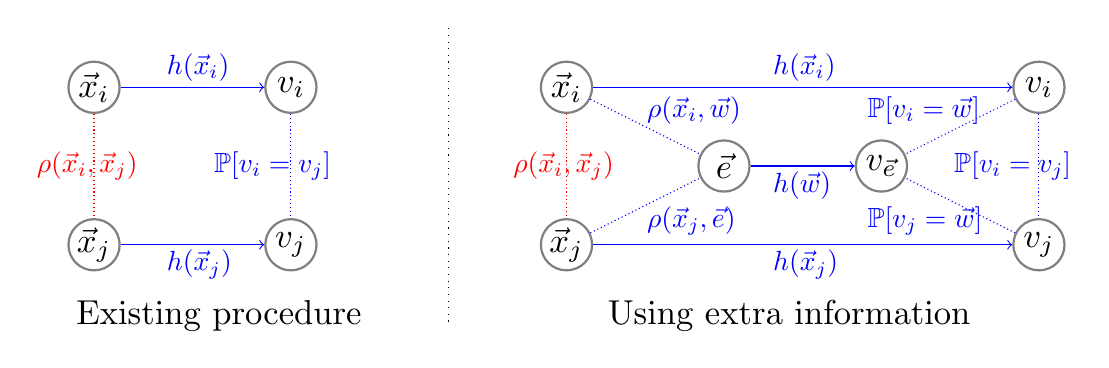
\begin{tikzpicture}
\tikzstyle{place}=[circle,draw=black!50,thick, inner sep=0pt,minimum size=6.5mm] 

\node at ( 0,0) [place] (xi) {$\Scale[1.25]{\vec{x}_i}$}; 
\node at ( 0,-2) [place] (xj) {$\Scale[1.25]{\vec{x}_j}$}; 


\node at ( 2.5,0) [place] (vi) {$\Scale[1.25] \vi$}; 

\node at ( 2.5,-2) [place] (vj) {$\Scale[1.25] \vj$}; 



\draw [densely dotted,red] (xi) -- (xj);
\draw [densely dotted,blue] (vi) -- (vj);

\draw[->,blue] (xi) -- (vi);
\draw[->,blue] (xj) -- (vj);

\coordinate [label=right:{\textcolor{blue}{$\Scale[1]{h(\vec{x}_i)}$}}] (A) at (8mm, 2.5mm); 

\coordinate [label=right:{\textcolor{blue}{$\Scale[1]{h(\vec{x}_j)}$}}] (A) at (8mm, -22.5mm); 

\coordinate [label=right:{\textcolor{blue}{$\Scale[1]{\mathbb P[v_i = v_j]} $}}] (A) at (14.0mm, -10mm); 

\coordinate [label=right:{\textcolor{red}{$\Scale[1]{\rho(\vec{x}_i,\vec{x}_j)}$}}] (A) at (-8.5mm, -10mm); 

\coordinate [label=right:{\Scale[1.25]{\text{Existing procedure}}}] (A) at (-3.5mm, -29mm); 



\draw[dotted] (4.5,0.75) -- (4.5,-3);

\node at ( 6,0) [place] (new_xi) {$\Scale[1.25]{\vec{x}_i}$}; 

\node at ( 6,-2) [place] (new_xj) {$\Scale[1.25]{\vec{x}_j}$}; 

\node at (8,-1) [place] (e) {$\Scale[1.25]{\vec{e}}$}; 
\node at (10,-1) [place] (ve) {$\Scale[1.25]{{v}_{\vec{e}}}$}; 


\node at ( 12,0) [place] (new_vi) {$\Scale[1.25]{{v}_i}$}; 

\node at ( 12,-2) [place] (new_vj) {$\Scale[1.25]{{v}_j}$}; 

\draw [densely dotted,red] (new_xi) -- (new_xj);

\draw [densely dotted,blue] (new_vi) -- (new_vj);
\draw[->,blue] (new_xi) -- (new_vi);
\draw[->,blue] (new_xj) -- (new_vj);
\draw[->,blue] (e) -- (ve);

\draw [densely dotted,blue] (new_xi) -- (e);
\draw [densely dotted,blue] (new_xj) -- (e);

\draw [densely dotted,blue] (new_vi) -- (ve);
\draw [densely dotted,blue] (new_vj) -- (ve);


\coordinate [label=right:{\textcolor{red}{$\Scale[1]{\rho(\vec{x}_i,\vec{x}_j)}$}}] (A) at (52mm, -10mm); 

\coordinate [label=right:{\textcolor{blue}{$\Scale[1]{h(\vec{x}_i)}$}}] (A) at (85mm, 2.5mm); 

\coordinate [label=right:{\textcolor{blue}{$\Scale[1]{h(\vec{x}_j)}$}}] (A) at (85mm, -22.5mm); 

\coordinate [label=right:{\textcolor{blue}{$\Scale[1]{h(\vec{w})}$}}] (A) at (85mm, -12.5mm); 

\coordinate [label=right:{\textcolor{blue}{$\Scale[1]{\mathbb P[v_i = v_j]}$}}] (A) at (108.0mm, -10mm); 



\coordinate [label=right:{\textcolor{blue}{$\Scale[1]{\rho(\vec{x}_i,\vec{w})}$}}] (A) at (69mm, -3mm); 

\coordinate [label=right:{\textcolor{blue}{$\Scale[1]{\mathbb P[v_i = \vecw]}$}}] (A) at (97mm, -3mm); 

\coordinate [label=right:{\textcolor{blue}{$\Scale[1]{\mathbb P[v_j = \vecw]}$}}] (A) at (97mm, -17mm); 

\coordinate [label=right:{\textcolor{blue}{$\Scale[1]{\dist{\vecxj}{\vece}}$}}] (A) at (69mm, -17mm); 

\coordinate [label=right:{\Scale[1.25]{\text{Using extra information}}}] (A) at (64mm, -29mm); 


\end{tikzpicture} 
\end{center}
\caption{\label{fig1}Using one extra vector $\vec{e}$ for which we know relevant information \blue{(shown in blue)} to estimate unknown $\rho(\vec{x}_i,\vec{x}_j)$ (shown in red).~\label{extra_info_pic}}
\end{figure*}

In the original LSH scheme, we know the hash function $h$ and its relation to $\mathbb P[v_i = v_j]$ \blue{(blue)}. We condition on these information to find $\rho(\vec{x}_i,\vec{x}_j)$ \red{(red)}.

In the extra information case, we generate an extra vector $\vec{e} \in \mathbb{R}^p$, then compute and store $\rho(\vec{x}_i, \vec{e}), 1 \leq i \leq n$. This takes $O(np)$ time and requires $O(n)$ space. We then compute the hashed values $v_i, 1 \leq i \leq n$ and $v_{\vec{e}}$. Finally, we condition on all of the known information \blue{(blue)} to estimate $\rho(\vec{x}_i,\vec{x}_j)$ \red{(red)}.
        
We now describe what happens in practice where we hash $k$ times. The hashed results are stored in a matrix $Y_{n+1, k}$, where the last row corresponds to the $k$ hashed values $h(\vec{e})$. We denote the last row as $Y_{e}$. 

We remark that the hashed values can be either discrete \cite{broder1997resemblance} or binary \cite{charikar2002similarity}, depending on the LSH scheme. The MLE approach \cite{kang2018improving} then considers the following sets for binary and discrete-typed hashes where:
\begin{align}
A := \{s \mid Y_{is} \neq Y_{js}, Y_{js} = Y_{es}\} ~~~~~ B := \{s \mid Y_{is} = Y_{js}, Y_{js} \neq Y_{es}\} \\
C := \{s \mid Y_{is} = Y_{js}, Y_{js} = Y_{es}\} ~~~~~ D := \{s \mid Y_{is} \neq Y_{js}, Y_{js} \neq Y_{es}\}
\end{align}
        is the collection of indices for binary hashes, $1 \leq s \leq k$ and
        \begin{align}
            &A := \{s \mid Y_{is} = Y_{js}, Y_{js} = Y_{es}\} \\
            &B := \{s \mid Y_{is} \neq Y_{js}, Y_{is} \neq Y_{es}, Y_{js} = Y_{es}\} \\
            &C := \{s \mid Y_{is} \neq Y_{js}, Y_{is} = Y_{es}, Y_{js} \neq Y_{es}\} \\
            &D := \{s \mid Y_{is} = Y_{js}, Y_{is} \neq Y_{es}, Y_{js} \neq Y_{es}\} \\
            &E := \{s \mid Y_{is} \neq Y_{js}, Y_{is} \neq Y_{es}, Y_{js} \neq Y_{es}\}
        \end{align}
        is the collection of indices for discrete hashes, $1 \leq s \leq k$.
        
        Then, let $n_i$ denote the cardinality of the set $i$, with $n_A + n_B + n_C + n_D = k$ for binary hashes, and $n_A + n_B + n_C + n_D + n_E = k$ for discrete hashes. Also, let $p_i$ be the probability that an observed element falls in set $i$.
        
       \subsection{Binary hashes}
        For any given observed cardinalities $n_A, n_B, n_C, n_D$, the likelihood of such an event, given parameters $p_A, p_B, p_C, p_D$, would be
\begin{align}
        \mathcal{L}(p_A, p_B, p_C, p_D) = \frac{k!}{n_A!n_B!n_C!n_D!} p_A^{n_A} p_B^{n_B} p_C^{n_C} p_D^{n_D}
\end{align}
        
However, as $\rho(\vec{x}_i, \vec{e})$ have been stored and computed, then we also have the following constraints
\begin{align}
p_A + p_C &= \rho(\vec{x}_j, \vec{e}) := p_{je} \label{cs1} \\
p_C + p_D &= \rho(\vec{x}_i, \vec{e}) := p_{ie} \label{cs2} \\
p_A + p_B + p_C + p_D &= 1 \label{cs3}
\end{align}
        
        Taking the log-likelihood and substituting in the above constraints, we obtain
\begin{equation}
        \begin{split}
        l(p_C) = K &+ n_A \log(p_{je} - p_C) + n_B \log(1 + p_C - p_{ie} - p_{je}) \\
        &+ n_C \log(p_C) + n_D \log(p_{ie} - p_C) \label{binary_cubic}
        \end{split}
\end{equation}
$\hat{p}_C$ can thus be expressed as a root of a cubic, as described in \cite{kang2018improving}, and found via numerical methods.

\subsection{Discrete hashes}
        The procedure for discrete hashes is similar. We have the same constraints, but since we now have five variables (instead of four in the binary case), we write our log-likelihood in terms of two variables, say $p_A$ and $p_D$ to obtain
        \begin{equation}
        \begin{split}
            l(p_A, p_D) = K &+ n_A \log(p_A) + n_B \log(p_{je}-p_A) + n_C \log(p_{ie} - p_A) \\
            &+ n_D \log(p_D) + n_E \log(1 - p_{ie} - p_{je} + p_A - p_D)
        \end{split} \label{discrete_cubic}
        \end{equation}
By calculus, we can express
\begin{align}
        p_D = \frac{n_D(1 + p_A - p_{ie} - p_{je})}{n_D + n_E}
\end{align}
and find $p_A$ expressed as a root of a cubic via numerical methods.

However, finding the root of these cubics are not numerically stable for low values of $k$, which leads us to consider a new estimator.

\section{Our Control Variate Estimator: Binary Hashes}

Suppose we have generated a random vector $\vec{e} \in \mathbb{R}^p$, and computed and stored the similarities $\rho(\vec{x}_i, \vec{e})$ for each observation, similar to the setup in \cite{kang2018improving,Kang2021-correlations}
        
        Now, suppose we want to estimate $p_{ij} = \rho(\vec{x}_i, \vec{x}_j)$ for any pair of observations $\vec{x}_i, \vec{x}_j$, and we have $k$ hashes. We define the following random variables
\begin{align}
A := \frac{\sum_{s=1}^k 1_{\{Y_{is} = Y_{js}\}}}{k} ~~~ B := \frac{\sum_{s=1}^k 1_{\{Y_{is} = Y_{es}\}}}{k} ~~~ C := \frac{\sum_s 1_{\{Y_{js} = Y_{es}\}}}{k}
\end{align}
        
        Then, $\mathbb{E}[A] = p_{ij}$, $\mathbb{E}[B] = \rho(\vec{x}_i, \vec{e})$ and $\mathbb{E}[C] = \rho(\vec{x}_j, \vec{e})$. We know $\mathbb{E}[B], \mathbb{E}[C]$ from pre-calculating $\rho(\vec{x}_i, \vec{e})$ and $\rho(\vec{x}_j, \vec{e})$.
        
We define the following new estimator:
        \begin{equation}\label{cv_est}
            A' = A + c_1(B - \e[B]) + c_2(C - \e[C])
        \end{equation}

$A'$ is an unbiased estimator of $p_{ij}$ and guaranteed to have a lower variance than $A$ as long as either (or both of) $\text{Cov}(A, B)$ and $\text{Cov}(A, C)$ are non-zero.
        
        By finding the partial derivative of $\text{Var}(A')$ and solving for optimal $\hat{c}_1, \hat{c}_2$, we can get the optimal control variate corrections. Thus, we have
        \begin{equation}
        \begin{split}
            \var(A') = &\var(A) + c_1^2\var(B) + c_2^2\var(C) + 2c_1 \cov(A, B) + 2c_2 \cov(A, C) \\
            &+ 2c_1 c_2 \cov(B, C)
        \end{split}
        \end{equation}

The partial derivatives are
        \begin{align}
            \frac{\partial\var(A')}{\partial c_1} = 2c_1\var(B) + 2\cov(A, B) + 2c_2\cov(B,C)\\
            \frac{\partial\var(A')}{\partial c_2} = 2c_2\var(C) + 2\cov(A, C) + 2c_1\cov(B,C)
        \end{align}
        
Denoting the covariance matrix between $B$ and $C$ as $\Sigma$, and packing the covariances $\cov(A,B), \cov(A,C)$ as a column vector $\Sigma_{A}$, we can write the equations forming the optimal values of $c_1$ and $c_2$ as follows: $[c_1~~c_2]^T = \Sigma^{-1} \Sigma_{A}$.
        
Now, the control variate corrections $c_1$ and $c_2$ involve the true value of $p_{ij}$ in the calculations of $\Sigma$ and $\Sigma_A$, which we do not have. To get around this, one solution is to obtain an initial estimate for $p_{ij}$ using $\frac{1}{k}\sum_{s=1}^k{A}$ similar to \cite{Kang2021-correlations}. Another solution involves finding analytic expressions for $\Sigma$ and $\Sigma_A$, collecting the $p_{ij}$ terms on one side, and finally solving the resultant cubic.
        
\begin{theorem}
Suppose we set $g(p_C)$ to be the cubic found after calculus in \eqref{binary_cubic} and $f(p_C)$ to be the cubic we find after our control variate approach. We have that $\frac{f(p_A)}{g(p_A)} = -2$.
\end{theorem}

\begin{proof}
We can write $A, B, C$ in our estimator as
\begin{align}
A = \frac{n_B + n_C}{k} ~~~~~ B = \frac{n_C + n_D}{k} ~~~~~ C = \frac{n_A + n_C}{k}
\end{align}
            
We set $A' = p_{ij}$, which we rewrite in terms of $p_C$ by using the result presented in \eqref{cs1}-\eqref{cs3}. Furthermore, as $A, B, C$ are Bernoulli random variables, we can easily calculate their expectations, variances and covariances as follows
\begin{align}
\e[A] &= p_{ij} = 1 + 2p_C - p_{ie} - p_{je} \\
\var(A) & = p_{ij} (1 - p_{ij}) = (1 + 2p_C - p_{ie} - p_{je})(p_{ie} + p_{je} - 2p_C)\\  
\e[B] &= p_{ie} \hspace{5.4cm} \e[C] = p_{je} \\
\var(B) &= p_{ie} (1 - p_{ie}) \hspace{3.7cm}\var(C) = p_{je} (1 - p_{je}) \\
                \cov(A, B) &= p_C - p_{ie}(1 + 2p_C - p_{ie} - p_{je})~~~~\cov(B, C) = p_C - p_{ie}p_{je} \\
                \cov(A, C) &= p_C - p_{je}(1 + 2p_C - p_{ie} - p_{je})            
            \end{align}
            
            We can then substitute all these rewritten expressions back into \eqref{cv_est}. By bringing $A'$ over, and cross-multiplying to remove the denominator, we obtain the following equation, which we call $f(p_C)$:
\begin{equation}\label{cvb_fin}
\begin{split}
f(p_C) ={} &- 2 n_{1} p_C^{3} + 4 n_{1} p_C^{2} p_{ie} + 2 n_{1} p_C^{2} p_{je} - 2 n_{1} p_C^{2} - 2 n_{1} p_C p_{ie}^{2} - 2 n_{1} p_C p_{ie} p_{je} \\
 &+ 2 n_{1} p_C p_{ie} - 2 n_{2} p_C^{3} + 2 n_{2} p_C^{2} p_{ie} + 2 n_{2} p_C^{2} p_{je} - 2 n_{2} p_C p_{ie} p_{je} - 2 n_{3} p_C^{3} \\
 &+ 4 n_{3} p_C^{2} p_{ie} + 4 n_{3} p_C^{2} p_{je} - 2 n_{3} p_C^{2} - 2 n_{3} p_C p_{ie}^{2} - 6 n_{3} p_C p_{ie} p_{je} + 2 n_{3} p_C p_{ie} \\
&- 2 n_{3} p_C p_{je}^{2} + 2 n_{3} p_C p_{je} + 2 n_{3} p_{ie}^{2} p_{je} + 2 n_{3} p_{ie} p_{je}^{2} - 2 n_{3} p_{ie} p_{je} - 2 n_{4} p_C^{3} \\
&+ 2 n_{4} p_C^{2} p_{ie} + 4 n_{4} p_C^{2} p_{je} - 2 n_{4} p_C^{2} - 2 n_{4} p_C p_{ie} p_{je} - 2 n_{4} p_C p_{je}^{2} + 2 n_{4} p_C p_{je}
                \end{split}
            \end{equation}
which is exactly equivalent to the $\frac{1}{2}$ of cubic in \cite{kang2018improving}.       
\end{proof}

\section{Our Estimator: Discrete Hashes}

Unlike the MLE approach for discrete hashes where we define a new collection of sets, our estimator uses the same random variables defined in the binary case.
        
We find that we require the true value of $p_{ij}$ to calculate $c_1$ and $c_2$. As such, we are presented with the same two options as in the binary case. We can either use $\frac{1}{k}\sum_s^k A$ as an initial estimate for $p_{ij}$, or we can collect the $p_{ij}$ terms on one side, and solve the root for the resultant cubic. Similarly, this result is equivalent to the cubic for discrete hashes.

\begin{theorem}
Suppose we set $g(p_A)$ to be the cubic found after calculus in \eqref{discrete_cubic} and $f(p_A)$ to be the cubic we find after our control variate approach. We have that $\frac{f(p_A)}{g(p_A)} = -2n_D - n_E$.
\end{theorem}

The equivalency of maximum likelihood estimation and control variates have been explored in \cite{glynn2002some} and \cite{szechtman2001constrained}, where they show how solving the ``constrained Monte Carlo" with non-parametric maximum likelihood estimation coincides with the method of control variates. This implies that the variance reduction for our control variate method is asymptotically equivalent to the variance reduction for maximum likelihood estimation method \cite{kang2018improving}.

However, the control variate method allows us to substitute in a proxy for $p_{ij}$ in our coefficients $c_1, c_2$ (or even compute the empirical covariance), rather than resorting than solving for a root of a cubic. This is less computationally costly than running Newton-Raphson. Moreover, Theorem 2 gives some (theoretical) insight why a naive implementation of the MLE estimator may not be numerically stable at low values of $k$, due to the values of $n_D$ and $n_E$, which may be zero for small $k$. 
 
\section{Application to Sign Random Projections}

We demonstrate how our estimator can be used for sign random projections (SRP). In SRP, we want an estimate for the angle $\theta_{ij}$ between any two vectors $\vec{x}_i$ and $\vec{x}_j$ \cite{goemans1995improved}. Given a data matrix $X_{n\times p}$, we generate a random matrix $R_{p\times k}$ with entries i.i.d from $N(0, 1)$. We next compute $V = \text{sgn}(XR)$ where we define $\text{sgn}(x) = 1_{\{x \geq 0\}}$. The estimate of $\theta_{ij}$ is given by $\hat{\theta} = \sum_{s=1}^k \frac{\pi}{k} \cdot 1_{\{V_{is} \neq V_{js}\}}$.
        
%        This can also be thought of as the Hamming distance between $\vec{v}_i$ and $\vec{v}_j$ multiplied by $\pi/k$.
        
Suppose we now generate an extra vector $\vec{e}$, similar to \cite{kang2018improving}. Then we only need to make minor modifications to our estimator to have it calculate estimates for the angles between two vectors. Specifically, we have $\e[A] = 1 - \frac{\theta_{ij}}{\pi}, \e[B] = 1 - \frac{\theta_{ie}}{\pi}$, and $ \e[C] = 1 - \frac{\theta_{je}}{\pi}$.
       
        
Computing $\e[AB] = \e[AC] = \e[BC]$ involves finding the ``three-way'' probability of $A$, $B$, and $C$. In the case of estimating angles, this is equivalent to having the three vectors $\vec{x}_i$, $\vec{x}_j$, and $\vec{e}$ fall on one side of some hyperplane. This probability is given by $1 - \frac{\theta_{ij} + \theta_{ie} + \theta{je}}{2\pi}$, with the proof given in \cite{kang2018improving}.

In general, in order to obtain estimates for any LSH scheme, we need to first obtain an expression for the ``three-way" probability of $A$, $B$, and $C$. In other words, we need to be able to calculate an expression for the expectation of the statistic $1_{\{Y_{is} = Y_{js} = Y_{es}\}}$. We discuss more on these in Section 8.

With the above modifications, our estimator is able to directly output an estimate of the angle between any two vectors.
        
        
\section{Experimental Results}

    We demonstrate our estimators by using the MNIST test dataset \cite{lecun1998gradient} and the Gisette dataset \cite{guyon2004result,Lichman:2013}. The MNIST test dataset has $n = 10,000$ observations with $p=784$ parameters. The Gisette dataset has $n=13,500$ observations with $p=5000$ parameters. We normalise the vectors in both datasets to unit length. To ensure reproducibility, we use a constant seed for our experiments. Furthermore, we set the extra vector $\vec{e}$ to be the mean vector across all observations in each dataset. The simulations are written in Python, and make use of GPU-accelerated computations through the library PyTorch. %The code, as well as the instructions for running it, can be found at XX.
    
    In order to prevent possible biases in picking ``good pairs'' of vectors, we choose to calculate all possible pairwise estimates for the full dataset. We then calculate the mean-squared error between each estimate and the actual value.
    
    We vary $k$ over the range of $\{10, 20, \dots, 100\}$, and for $k$, we calculate and average the results over 100 iterations. For each individual simulation run, we calculate 4 different estimates, namely \verb|CV_SUB|, \verb|CV_CUBIC|, \verb|MLE|, and \verb|SRP|. Respectively, they refer to: using an initial estimate for the default control variate procedure, solving the cubic derived from control variates, solving the cubic derived from MLEs \cite{kang2018improving}, and sign random projections \cite{goemans1995improved}.
    
    We compute the average of all mean-squared errors of $49,995,000$ pairwise angular similarity estimates for the MNIST test dataset, as well as the average mean-squared errors of $91,118,250$ pairwise angular similarity estimates for the Gisette dataset. These are displayed in Figures \ref{mnist:mean} and \ref{gisette:mean} respectively. %\footnote{Higher-resolution versions of the images, as well as the data used to generate these images, can be found \href{https://github.com/Mickey1356/weighted-vecs/tree/main/final}{here}}.
        \begin{figure}
        \centering
        \begin{minipage}{.45\columnwidth}
            \centering
            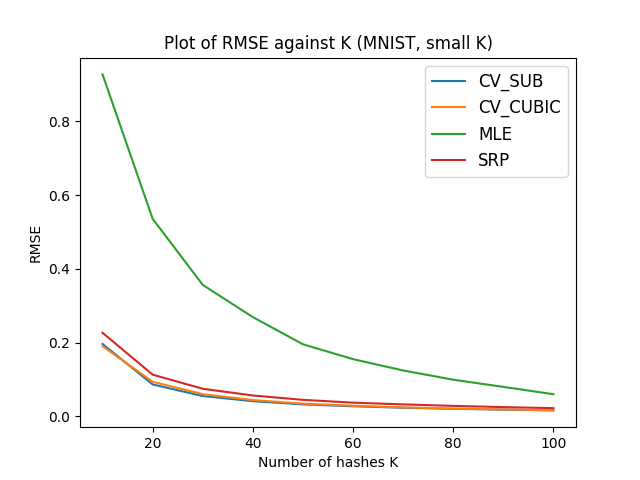
\includegraphics[width=\textwidth]{images/mnist_normal_mean.png}
            \caption{Averaged MSE for MNIST test dataset}
            \label{mnist:mean}
        \end{minipage}
        \hfill
        \begin{minipage}{.45\columnwidth}
            \centering
            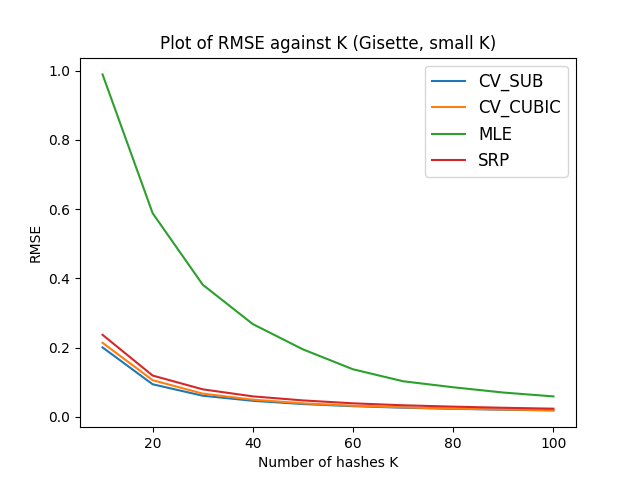
\includegraphics[width=\textwidth]{images/gisette_normal_mean.png}
            \caption{Averaged MSE for Gisette dataset}
            \label{gisette:mean}
        \end{minipage}
    \end{figure}
    % \begin{figure}[h]
    %     \centering
    %     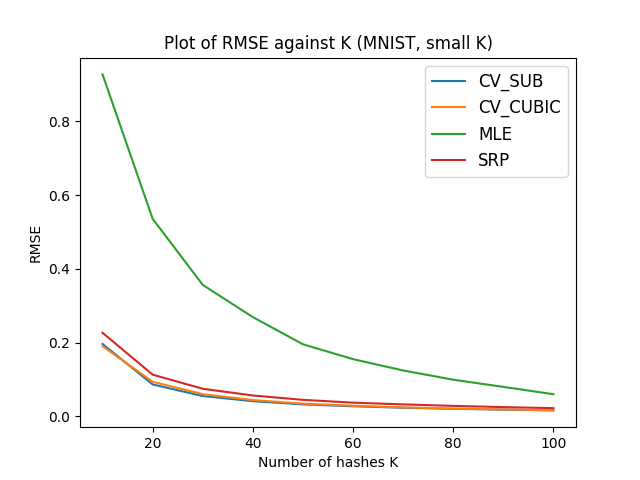
\includegraphics[width=0.25\textwidth]{images/mnist_normal_mean.png}
    %     \caption{Averaged mean-squared error for MNIST test dataset}
    %     \label{mnist:mean}
    % \end{figure}
    
    % \begin{figure}[h]
    %     \centering
    %     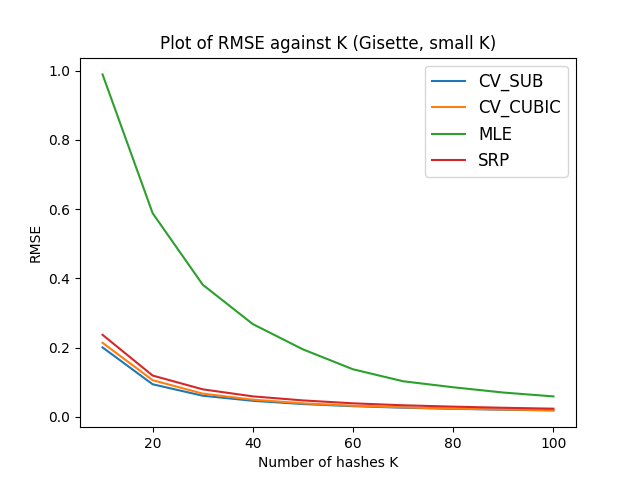
\includegraphics[width=0.25\textwidth]{images/gisette_normal_mean.png}
    %     \caption{Averaged mean-squared error for Gisette test dataset}
    %     \label{gisette:mean}
    % \end{figure}    
    In general, we note that \verb|CV_SUB| and \verb|CV_CUBIC| both consistently outperform \verb|SRP| and \verb|MLE|. Furthermore, we also note that \verb|CV_SUB|, that is, simply improving an initial estimate using control variates, outperforms solving the cubic in \verb|CV_CUBIC|. Finally, although \verb|CV_CUBIC| and \verb|MLE| have been shown to be equivalent in the previous sections, empirical results show that the control variates approach offers greater stability and accuracy compared to the MLE approach.

    This is because the calculation for \verb|MLE| relies on $n_A, n_B, n_C, n_D$. If any of them are zero due to few observations, this may result in a division-by-zero error. Cross-multiplying can help prevent this error, but the numerical stability would still be affected. On the other hand, \verb|CV_SUB| uses the empirical value of the control variate coefficient $c$. This takes the correlation of the already observed vectors into account, thus giving more accurate and stable results.
    
    We also plot the standard deviation of the mean-squared errors in Figures \ref{mnist:stddev} and \ref{gisette:stddev}. We note that \verb|CV_SUB| tends to have lower standard deviations compared to other estimates. We also note that for larger values of $k$, we can observe lower variances and higher accuracies compared to the baseline of \verb|SRP|.  
      \begin{figure}
        \centering
        \begin{minipage}{.45\columnwidth}
            \centering
            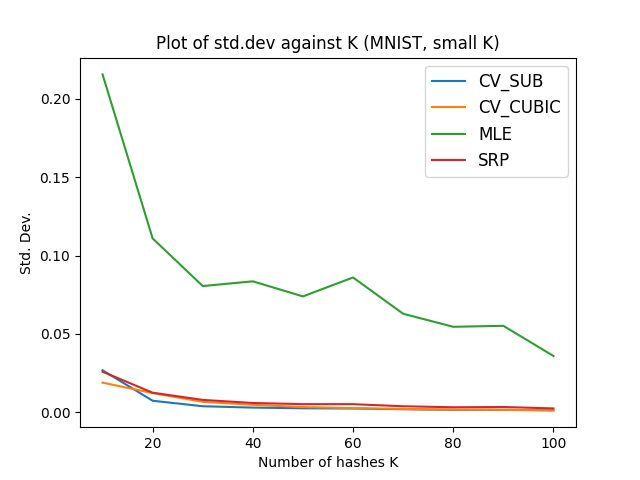
\includegraphics[width=\textwidth]{images/mnist_normal_stddev.png}
            \caption{Standard deviations for MNIST test dataset}
            \label{mnist:stddev}
        \end{minipage}
        \hfill
        \begin{minipage}{.45\columnwidth}
            \centering
            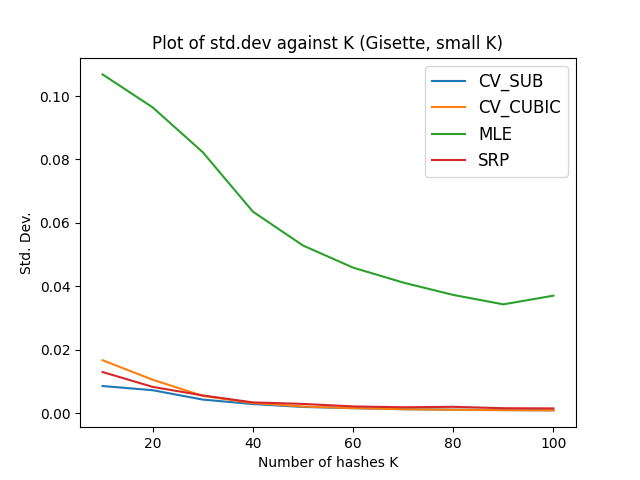
\includegraphics[width=\textwidth]{images/gisette_normal_stddev.png}
            \caption{Standard deviations for Gisette dataset}
            \label{gisette:stddev}
        \end{minipage}
    \end{figure}
    % \begin{figure}[h]
    %     \centering
    %     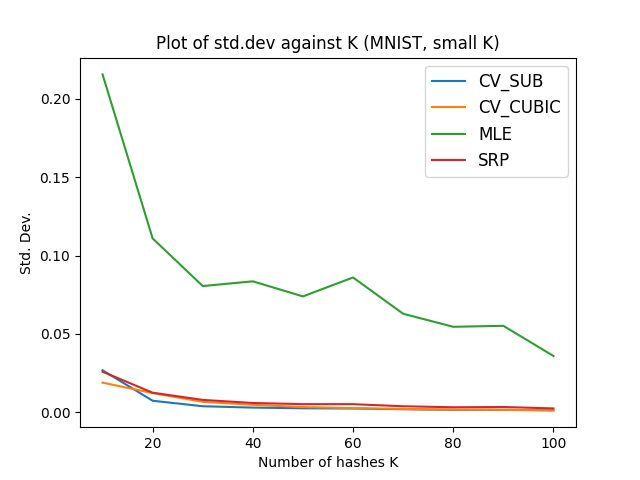
\includegraphics[width=0.25\textwidth]{images/mnist_normal_stddev.png}
    %     \caption{Standard deviations for MNIST test dataset}
    %     \label{mnist:stddev}
    % \end{figure}
    
    % \begin{figure}[h]
    %     \centering
    %     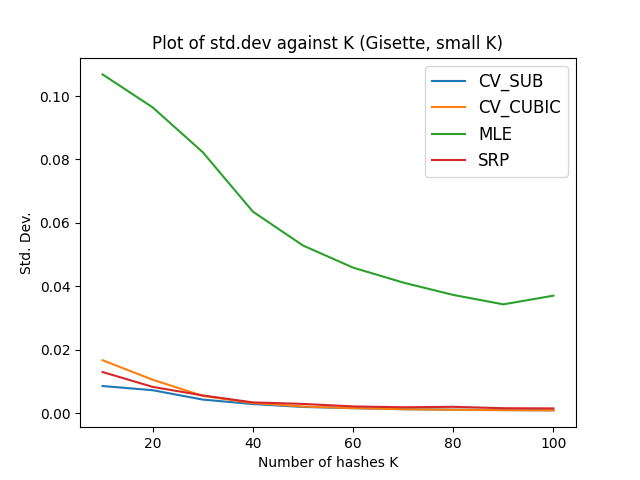
\includegraphics[width=0.25\textwidth]{images/gisette_normal_stddev.png}
    %     \caption{Standard deviations for Gisette test dataset}
    %     \label{gisette:stddev}
    % \end{figure}
    We also run another set of simulations for a wider range of $k = \{200, 250, \dots 1000\}$, to show the asymptotic behaviour of the estimators for larger values of $k$. This time, the results are obtained by averaging over 25 iterations. Again, we calculate these values from all possible pairs of vectors in both the MNIST and Gisette dataset. The results are graphed and displayed in Figures \ref{mnist:large} and \ref{gisette:large} for the MNIST and Gisette dataset respectively.
% \begin{center}
%     \setlength{\tabcolsep}{0.5em}
%     \begin{table}[h]
%         \centering
%         \caption{Average MSE for $k = 50$ and $k=1000$ (MNIST dataset)}
%         \label{table:mnist}
%         \begin{tabular}{|c|c|c|}
%             \hline & $k=50$ & $k=1000$  \\ \hline
%         \verb|SRP|       & $0.0448 \pm 0.0153$           & $0.00216 \pm 0.000381$          \\ \hline
%         \verb|MLE|       & $0.195 \pm 0.222$             & $0.00165 \pm 0.000205$          \\ \hline 
%         \verb|CV_SUB|    & $\mathbf{0.0324 \pm 0.00731}$ & $\mathbf{0.00163 \pm 0.000180}$ \\ \hline
%         \verb|CV_CUBIC|  & $0.0345 \pm 0.00974$          & $0.00164 \pm 0.00974$            \\ \hline
%         \end{tabular}%
%     \end{table}
%     \begin{table}[h]
%         \centering
%         \caption{Average MSE for $k = 50$ and $k=1000$ (Gisette dataset)}
%         \label{table:gisette}
%         \begin{tabular}{|c|c|c|}
%             \hline & $k=50$ & $k=1000$  \\ \hline
%         \verb|SRP|        & $0.0477 \pm 0.00867$           & $0.002400 \pm 0.000498$ \\ \hline
%         \verb|MLE|        & $0.195 \pm 0.159$              & $0.00192 \pm 0.000107$ \\ \hline 
%         \verb|CV_SUB|     & $\mathbf{0.0372 \pm 0.00578}$  & $\mathbf{0.00192 \pm 0.000119}$ \\ \hline
%         \verb|CV_CUBIC|   & $0.0393 \pm 0.00621$           & $0.00192 \pm 0.000107$ \\ \hline
%         \end{tabular}%
%     \end{table}
% \end{center}
\begin{center}
    \begin{table}[h]
        \small
        \centering
        \caption{Average MSE for $k = 50$ and $k=1000$}
        \label{table:small_k}
        \begin{adjustbox}{width=\columnwidth,center}
        \begin{tabular}{|c|c|c|c|c|}
        \hline & \textbf{MNIST} ($k=50$) & \textbf{Gisette} ($k=50$) & \textbf{MNIST} ($k=1000$) & \textbf{Gisette} ($k=1000$)  \\ \hline
        \verb|SRP|       & $0.0448 \pm 0.0153$ & $0.0477 \pm 0.00867$ & $0.00216 \pm 0.000381$ & $0.002400 \pm 0.000498$ \\ \hline
        \verb|MLE|       & $0.195 \pm 0.222$ & $0.195 \pm 0.159$ & $0.00165 \pm 0.000205$ & $0.00192 \pm 0.000107$ \\ \hline 
        \verb|CV_SUB|    & $\mathbf{0.0324 \pm 0.00731}$ & $\mathbf{0.0372 \pm 0.00578}$ & $\mathbf{0.00163 \pm 0.000180}$ & $\mathbf{0.00192 \pm 0.000119}$ \\ \hline
        \verb|CV_CUBIC|  & $0.0345 \pm 0.00974$ & $0.0393 \pm 0.00621$  & $0.00164 \pm 0.00974$ & $0.00192 \pm 0.000107$ \\ \hline
        \end{tabular}
        \end{adjustbox}
    \end{table}
\end{center}    
    We observe that \verb|MLE| only outperforms \verb|SRP| for larger values of $k$, but does not match the performance of control variate. We also observe that as $k$ increases, \verb|MLE| asymptotically approaches the same performance as \verb|CV_CUBIC|. This verifies the equivalency of the two approaches as proven in Theorems 1 and 2.    
    \begin{figure}
        \centering
        \begin{minipage}{.45\columnwidth}
            \centering
            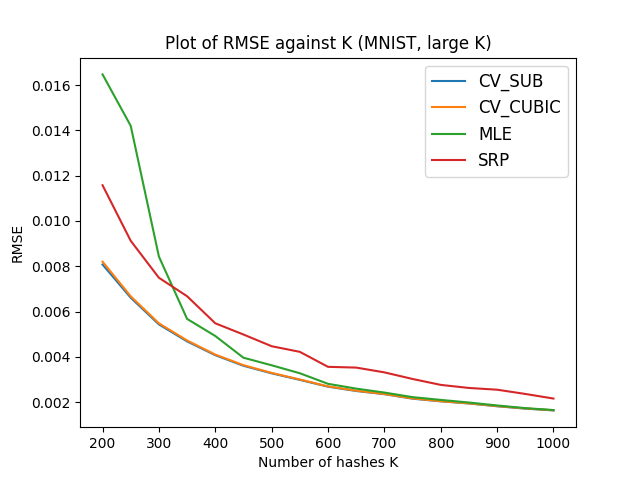
\includegraphics[width=\textwidth]{images/mnist_large_mean.png}
            \caption{Averaged MSE for MNIST test dataset}
            \label{mnist:large}
        \end{minipage}
        \hfill
        \begin{minipage}{.45\columnwidth}
            \centering
            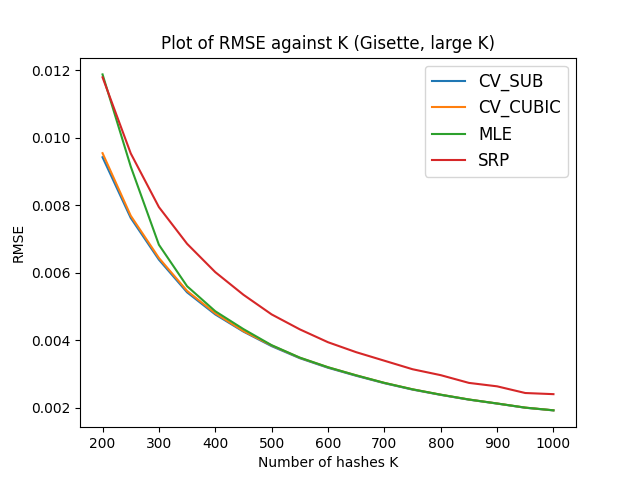
\includegraphics[width=\textwidth]{images/gisette_large_mean.png}
            \caption{Averaged MSE for Gisette dataset}
            \label{gisette:large}
        \end{minipage}
    \end{figure}
    Table \ref{table:small_k} displays the averaged MSE (with bounds of 3 standard deviations) for $k=50$ and $k = 1000$ for both the MNIST and Gisette datasets. We can see that for both datasets, the MSE for \verb|MLE| and \verb|CV_CUBIC| are approximately equal at $k = 1000$, verifying that our two methods are asymptotically identical.
    
    We note that although large values of $k$ give higher accuracies, it does not make sense to use values of $k$ which are similar in magnitude to the original dimensions of the data, $p$. This is because the computational complexities of our estimators are in the order of $O(n^2k)$, while the computational complexity of calculating each pairwise angle is $O(n^2p)$. Using larger values of $k$ would result in a slower running time, due to the additional overhead of preprocessing the hash values. In this sense, we are only interested in the results for small values of $k$, but nevertheless, our CV approach still matches/outperforms the MLE approach even for large $k$.

    To verify this, we display the average running time of the various algorithms for $k=\{50, 500, 1000\}$ on the MNIST dataset in Table \ref{table:timings}. As expected, for small $k$, all estimators are faster than directly calculating the angles, but this changes as $k$ increases. We note that \verb|SRP| is the fastest, with our estimator, \verb|CV_SUB| coming in close second. There is a tradeoff between accuracy and efficiency, but because both algorithms keep to the same order of complexity, the time tradeoff is not too significant. On the other hand, due to the need to numerically solve a cubic (through Newton-Raphson), \verb|CV_CUBIC| and \verb|MLE| have a much more noticeable accuracy-efficiency tradeoff.
        \begin{table}[h]
            \small
            \centering
            \caption{Average time taken (in seconds) for $k = \{50,500,1000\}$ on MNIST dataset}
            \label{table:timings}
            \begin{tabular}{|c|c|c|c|}
                \hline             & $k=50$ & $k=500$ & $k=1000$ \\ \hline
                Direct Calculation & \multicolumn{3}{c|}{$135.3$}      \\ \hline
                \verb|SRP|         & $11.28$   & $138.4$    & $287.4$     \\ \hline
                \verb|MLE|         & $99.05$   & $881.5$    & $1805$     \\ \hline 
                \verb|CV_SUB|      & $15.20$   & $146.7$    & $294.9$     \\ \hline
                \verb|CV_CUBIC|    & $47.38$   & $181.1$    & $335.3$     \\ \hline
            \end{tabular}
        \end{table}
    Overall, our results shows that our control variate estimator, not only offers an increase in accuracy from the baseline of \verb|SRP|, but also consistently outperforms the MLE approach proposed by \cite{kang2018improving}.
    
\section{Discussion on Control Variates}
    
    An added benefit of using control variates is the ability to easily extend to include additional extra vectors. For example, we can generate further extra vectors $\vec{e}_1, \vec{e}_2, \dots \vec{e}_j$, which can also be used to obtain even more accurate estimates.
    
    For each extra vector $e_t$, we first pre-compute and store $\rho(\vec{x}_i, \vec{e}_t)$ for all observations. Then we have the following random variables for each extra vector:
    \begin{align}
A := \frac{\sum_s 1_{\{Y_{is} = Y_{js}\}}}{k} ~~~~~ B_t := \frac{\sum_s 1_{\{Y_{is} = Y_{e_ts}\}}}{k} ~~~~~ C_t := \frac{\sum_s 1_{\{Y_{js} = Y_{e_ts}\}}}{k}
\end{align}
    
We can disregard the additional random variables of the form $1_{\{Y_{e_ms} = Y_{e_ns}\}}$ because their covariance with $A$ is 0. In general, for any two random variables to have a non-zero covariance, they must share at least one vector in common. Because we are interested in reducing the variance of $A$, any random variable we consider should at least share a common vector with $A$.
 
    Thus, we can define the new estimator of $A'$ of $p_{ij}$ as follows:
    \begin{align}
        A' = A + \sum_{t=0}^j c_{t,1}(B_t - \e[B_t]) + c_{t,2}(C_t - \e[C_t])
    \end{align}

    Minimising \var($A'$), we obtain the following system of equations for $\vec{c}$:
    \begin{align}
        \begin{bmatrix}
                c_{1,1}& c_{1,2} & \dots & c_{j, 1} & c_{j, 2}
        \end{bmatrix}^T = \Sigma^{-1} \Sigma_{A}
    \end{align}
    where $\Sigma$ refers to the covariance matrix of the random vector $\mathbf{X}$ whose elements are $(B_1, C_1, \dots B_j, C_j)^T$, and $\Sigma_{A}$ refers to the column vector whose elements are the covariances of $\mathbf{X}$ with respect to $A$.
    
    In order to solve the system of equations above, we would need the covariance matrices. Since $\cov(X,Y) = \e[XY] - \e[X]\e[Y]$, and we already have $\e[X]$ and $\e[Y]$, we would only need to find expressions for $\e[XY]$.
    
    Now, $B_t$ and $C_t$ are random variables that relate how two vectors are similar to one another. Thus, the expectation $\e[B_iC_j]$ for any $i,j$ rely on which vectors are being referred to. If they share a common vector, such that the three vectors in question are $\vec{x}$, $\vec{y}$ and $\vec{z}$, then the product becomes finding the expectation of the random variable $1_{\{Y_{xs} = Y_{ys} = Y_{zs}\}}$. This is the ``three-way'' similarity between the three vectors. For sign random projections, this is the probability that the three vectors lie on the same side of a hyperplane.
    
    If the random variables do not share any common vectors, e.g. $B_1$ and $C_2$, then, their covariance would equal to 0. This would mean that in the covariance matrix $\Sigma$ above, there are several entries which we would know to be 0. This makes our covariance matrix sparse, and hence computationally easier to compute the control variate coefficients.
    
We give an example of the covariance matrix $\Sigma$ for $j=4$ extra vectors:
    \begin{equation}
        \begin{blockarray}{ccccccccc}
            & B_1 & C_1 & B_2 & C_2 & B_3 & C_3 & B_4 & C_4\\
            \begin{block}{c[cc|cc|cc|cc]}
                B_1 & v & c & c & 0 & c & 0 & c & 0 \\
                C_1 & c & v & 0 & c & 0 & c & 0 & c \\
                \cmidrule(lr){2-9}
                B_2 & c & 0 & v & c & c & 0 & c & 0 \\
                C_2 & 0 & c & c & v & 0 & c & 0 & c \\
                \cmidrule(lr){2-9}
                B_3 & c & 0 & c & 0 & v & c & c & 0 \\
                C_3 & 0 & c & 0 & c & c & v & 0 & c \\
                \cmidrule(lr){2-9}
                B_4 & c & 0 & c & 0 & c & 0 & v & c \\
                C_4 & 0 & c & 0 & c & 0 & c & c & v \\
            \end{block}
        \end{blockarray}
    \end{equation}
    where $v, c$ are the respective variances and covariances to be calculated.
    
\section{Conclusion}
    We have shown how to use control variates to construct estimators for similarity estimation under LSH schemes. We have also demonstrated how our estimator could be used for sign random projections. The empirical results also show that our control variates estimator outperforms other estimators that use extra vectors to improve accuracy. Furthermore, we have shown how our estimator can easily be extended to include greater numbers of extra vectors, which would otherwise require redefining of contingency tables in other approaches.
    
    We believe that this strategy of using control variates can help improve estimates of vector similarities. The stability and accuracy at even low values of $k$ is an added improvement over other similar approaches. Hence, we believe that our framework of using control variates to achieve variance reduction could be beneficial when both fast computation and high accuracy is wanted.

\section{Acknowledgements}
    This work is funded by the Singapore Ministry of Education Academic Research Fund Tier 2 Grant MOE2018-T2-2-013, as well as with the support of the Singapore University of Technology and Design's Undergraduate Research Opportunities Programme.

    The authors also thank the anonymous reviewers for their comments and suggestions for improvement, which has helped to enhance the quality of the paper.
% table captions should be above
%
% ---- Bibliography ----
%
% BibTeX users should specify bibliography style 'splncs04'.
% References will then be sorted and formatted in the correct style.
%
\bibliographystyle{splncs04}
\bibliography{bib}
%


\end{document}
